%%%%%%%%%%%%%%%%%%%%%%%%%%%%%%%%%%%%%%%%%%%%%%%%%%%%%%%%%%%%%%%%%%%%%%%%%%%%%%
\section{$\pi^- p \to n \gamma$ photons as a calibration line}

Photons from RPC on hydrogen could be used to calibrate the Mu2e momentum scale and, simultaneously, measure the momentum resolution.
Consider a RPC  photon converting in the detector material 
and producing an $e^+e^-$ pair. In case of a symmetric conversion, the momenta of both particles
are $\sim$ 65 MeV/c. If the conversion radius is large enough, both an electron
and a positron from $\gamma \to e^+ e^-$ may produce enough hits in the tracker
so their tracks could be reconstructed and used to reconstruct the momentum of the
converted photon.

Acceptance is maximized for photons emitted at $90^o$ with respect to the DS axis. 

The Mu2e detector has a component, the pion degrader, which with small modifications
could be used for this calibration measurement. The degrader was initially introduced
in order to suppress the background to \piplusenu\ from muon decays
in flight \cite{MU2E_2527_PIPLUSENU},
It is a movable disk made of non-magnetic material, which gets inserted into
the beam during the calibration runs and moved out of the beam during
the regular data taking.

Making the degrader disk out of polyethylene and surrounding it, at a larger radius, 
with a thin converter foil could allow to convert photons emitted at angles close to $90^o$
with respect to the DS axis. A schematic view of the modified degrader geometry is presented in Figure~\ref{figure:degrader_geometry_v3}.

The converter foil could be supported by a light carbon foam disk mounted on the degrader.

\begin{figure}[H]
  \begin{tikzpicture}
    \node[anchor=south west,inner sep=0] at (0,-10.) {
      % \node[shift={(0 cm,0.cm)},inner sep=0,rotate={90}] at (0,0) {}
      \makebox[\textwidth][c] {
        \includegraphics[width=0.95\textwidth]{pdf/degrader_geometry_002}
      }
    };
    % \node [text width=8cm, scale=1.0] at (14.5,0.5) {$\mu_B$, expected background mean};
    % \node [text width=8cm, scale=1.0, rotate={90}] at (1.5,7.5) { $S_{D}$, ``discovery'' signal strength  };
  \end{tikzpicture}
  \caption{
    \label{figure:degrader_geometry_v3}
    Schematic view of the simulated degrader geometry, not up to scale
  }
\end{figure}

%%%%%%%%%%%%%%%%%%%%%%%%%%%%%%%%%%%%%%%%%%%%%%%%%%%%%%%%%%%%%%%%%%%%%%%%%%%%%%
\subsection{Simulation} 
A configuration of the Mu2e detector with the pion degrader, as shown in  Figure~\ref{figure:degrader_geometry_v3}, inserted in the beam has been simulated.

\begin{itemize}
\item 
  From \piplusenu\ studies: the pion degrader disk thickness of 4 mm Ti is close to optimal.
\item
  4mm of Ti translates into the total amount of material of $\sim 1.8 g/cm^2$,
  about twice the material of the stopping target.
\item
  9mm CH2 + 1.0mm Pb: : 2.0 $g/cm^2$   .. $\pi*15^2*(0.9*0.95 + 0.08*11.34): \simeq 2 g/cm^2$
\item
   9mm CH2 + 0.8mm Pb: : $1.76 g/cm^2$
 \item
   CH2 disk R=14 cm, weight        : $0.90*0.95*\pi*14^2 ~= 526$ gr \\
   Pb  foil R=10cm thickness 0.8mm : $0.08*11.34*\pi*10^2 = 285$ gr \\
   total                           : 811 gr
 \item 
   The gold converter ring has the outer radius $R_{out}$ = 250mm,
   and the value of $R_{in}$ is defined by the converter thickness.
   The converter is slightly offset downstream with respect to the $CH_2$ disk,
   so $e*+$ and $e^-$ produced in the converter do not cross it multiple times.

\end{itemize}

For small, of the order of few cm, widths of the converter ring,
the acceptance is proportional to the width.
So making teh width, for example, 3cm instead of 1 cm wide would increase
the acceptance by a factor close to x3. However, the space between the OPA
and the TS available
for the degrader installation is limited, about 5 cm along the Z axis, 
and that limits the maximal width of the converter ring. Also, a large radius
of the converter ring, R = 25-30 cm, could start limiting the movement of the
degrader arm.

A potentially more attractive alternative could be to have the converter placed
on a thin carbon foam ring and supported inside the OPA. In this case,
the width of the foil could be increased without introducing the space conflicts.
Having the converter supported by the OPA would also simplify increasing
the converter radius should that become necessary.
%
This option is discussed in Section~\ref{section:geometry_v4}


%%%%%%%%%%%%%%%%%%%%%%%%%%%%%%%%%%%%%%%%%%%%%%%%%%%%%%%%%%%%%%%%%%%%%%%%%%%%%%
\subsection{Stopped negative pions}

Simulation of the negative pion beam follows the standard 2-stage model.
Stage 2 produces three separate datasets of pions stops in the CH2, Pb, and the ST.
The scheme allow to resimulate the pion stop datasets w/o repeating more time consuming
first stage of the simulation.
To improve the simulation efficiency pion decays are disabled. The calculated by Geant4
pion survival probabilities are used as event weights in the normalization procedure.

Distributions of momentum and time for pions stopped in it CH2, Pb foil, and the
stopping target are shown in Figure \ref{figure:stopped_pim_mom_time}.

\begin{figure}[H]
  \begin{tikzpicture}
    \node[anchor=south west,inner sep=0] at (0,0.) {
      % \node[shift={(0 cm,0.cm)},inner sep=0,rotate={90}] at (0,0) {}
      % \makebox[\textwidth][c] {
        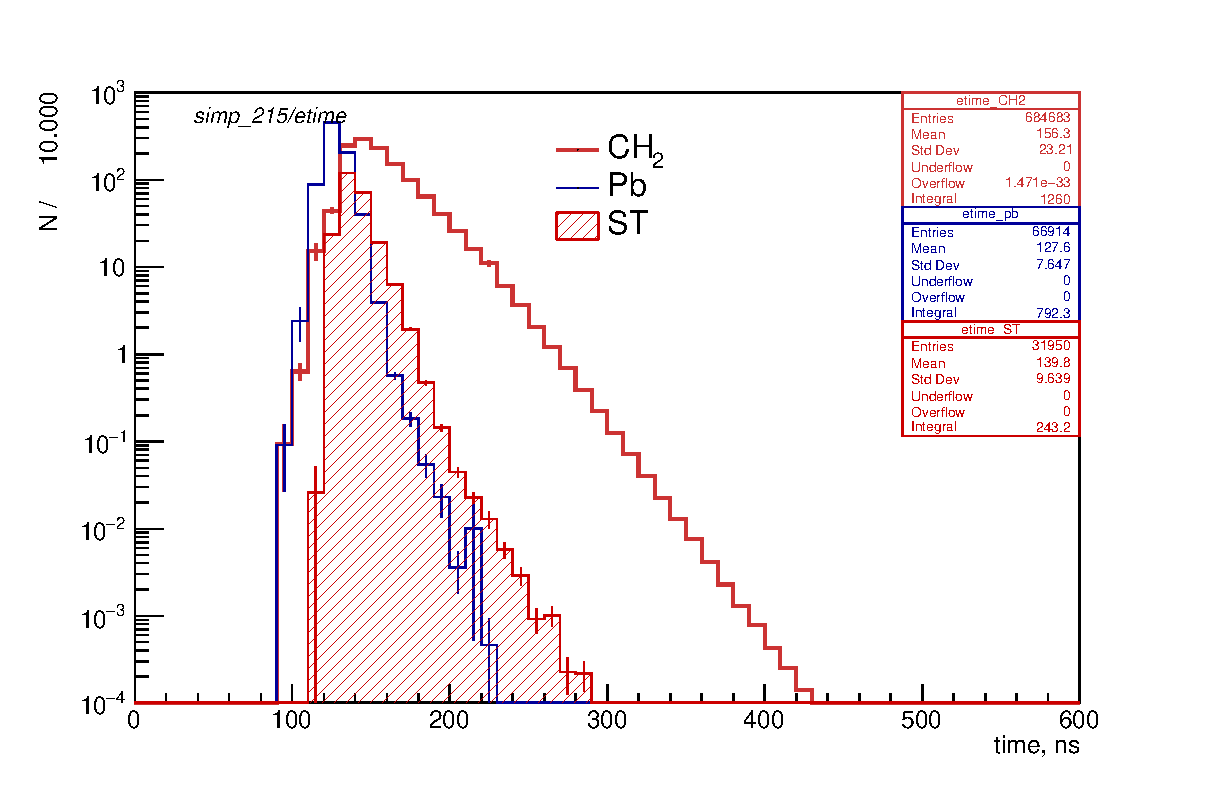
\includegraphics[width=0.5\textwidth]{pdf/figure_00021}
      % }
    };
    \node[anchor=south west,inner sep=0] at (10,0.) {
      % \node[shift={(0 cm,0.cm)},inner sep=0,rotate={90}] at (0,0) {}
      % \makebox[\textwidth][c] {
        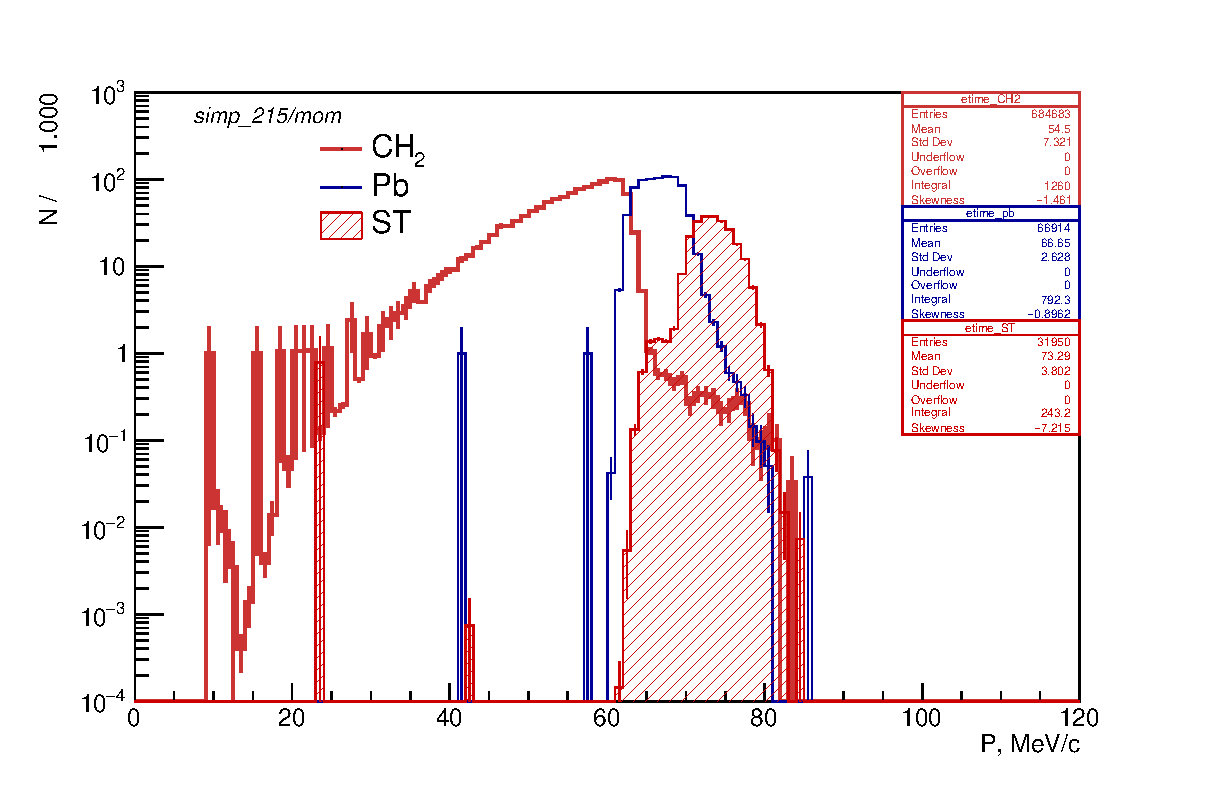
\includegraphics[width=0.5\textwidth]{pdf/figure_00022}
      % }
    };
    % \node [text width=8cm, scale=1.0] at (14.5,0.5) {$\mu_B$, expected background mean};
    % \node [text width=8cm, scale=1.0, rotate={90}] at (1.5,7.5) { $S_{D}$, ``discovery'' signal strength  };
  \end{tikzpicture}
  \caption{
    \label{figure:stopped_pim_mom_time}
    Stopped pions: distributions of momentum and time
  }
\end{figure}

It is worth noting that pions stopped in the $CH_2$ are the slowest ones.
Therefore, selecting events with the pion stop time above certain threshold, i.e. $\sim 200$ ns, 
significantly suppresses contributions of the stopping target and the Pb foil to any measurement.
T0 = 200 ns is also approximately the time where the instantaneous beam flash
hit rate gets reduced down to the level allowing the measurements. For the DAQ operations,
that means that the digitization start time should be lowered to $\sim 250$ ns,
which, at a reduced proton beam intensity, looks quite realistic.

Another interesting correlation is the correlation between the pion momentum on exit from the TS momentum
and the vertical coordinate of the pion stop point. Figure ~\ref{figure:y_vs_p_deg} shows this correlation
for pions stopped in the $CH_2$ and Pb parts of the degrader. The Y distribution of the pion stops
in the Pb foil is offset down by several centimeters. The lower cut-off at R=100 mm is determined by the
by the simulated radius of the Pb foil, R=100mm

\begin{figure}[H]
  \begin{tikzpicture}
    \node[anchor=south west,inner sep=0] at (0,0.) {
      % \node[shift={(0 cm,0.cm)},inner sep=0,rotate={90}] at (0,0) {}
      %\makebox[\textwidth][c] {
        \includegraphics[width=0.5\textwidth]{png/figure_00036}
      %}
    };
    \node[anchor=south west,inner sep=0] at (10.,0.) {
      % \node[shift={(0 cm,0.cm)},inner sep=0,rotate={90}] at (0,0) {}
      % \makebox[\textwidth][c] {
      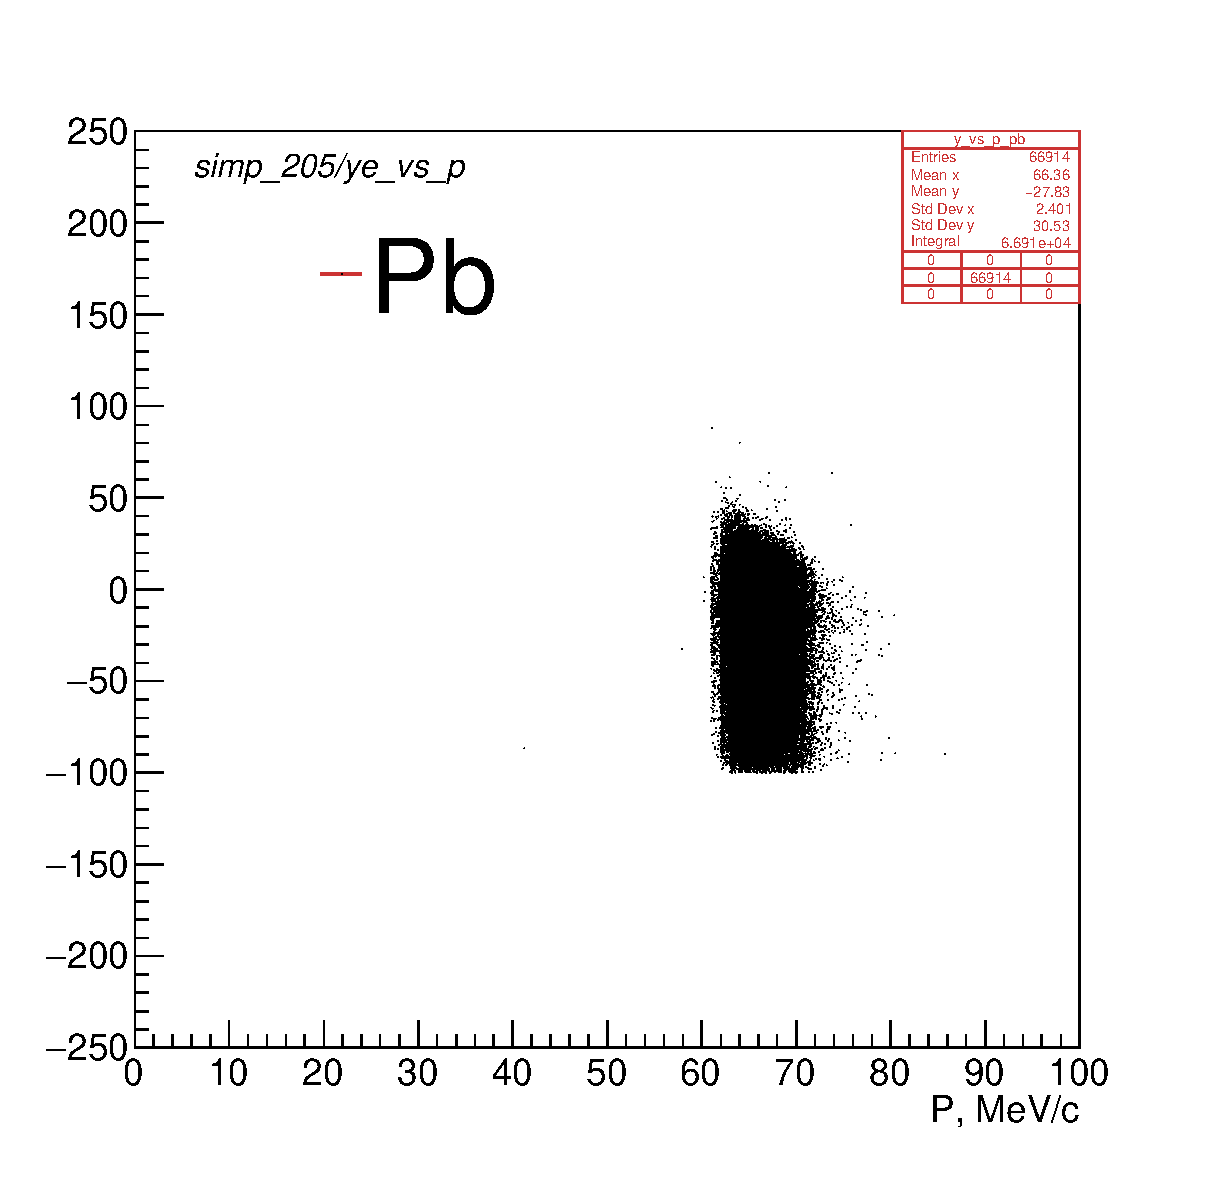
\includegraphics[width=0.5\textwidth]{png/figure_00037}
      %} 
    };
    % \node [text width=8cm, scale=1.0] at (14.5,0.5) {$\mu_B$, expected background mean};
    % \node [text width=8cm, scale=1.0, rotate={90}] at (1.5,7.5) { $S_{D}$, ``discovery'' signal strength  };
  \end{tikzpicture}
  \caption{
    \label{figure:y_vs_p_deg}
    Y(stop):P\@(DS entrance) for negative pions stopped in the $CH_2$ and Pb parts of the simulated degrader
  }
\end{figure}

Y:X distributions of the pion stops in the $CH_2$ disk, Pb foil and the ST are shown in Figure ~\ref{figure:y_vs_x_st}.
They reflect the correlation between the mean Y of the particle trajectory and the particle momentum.

\begin{figure}[H]
  \begin{tikzpicture}
    \node[anchor=south west,inner sep=0] at (0,0.) {
      % \node[shift={(0 cm,0.cm)},inner sep=0,rotate={90}] at (0,0) {}
      %\makebox[\textwidth][c] {
        \includegraphics[width=0.5\textwidth]{png/figure_00034}
      %}
    };
    \node[anchor=south west,inner sep=0] at (10.,0.) {
      % \node[shift={(0 cm,0.cm)},inner sep=0,rotate={90}] at (0,0) {}
      %\makebox[\textwidth][c] {
        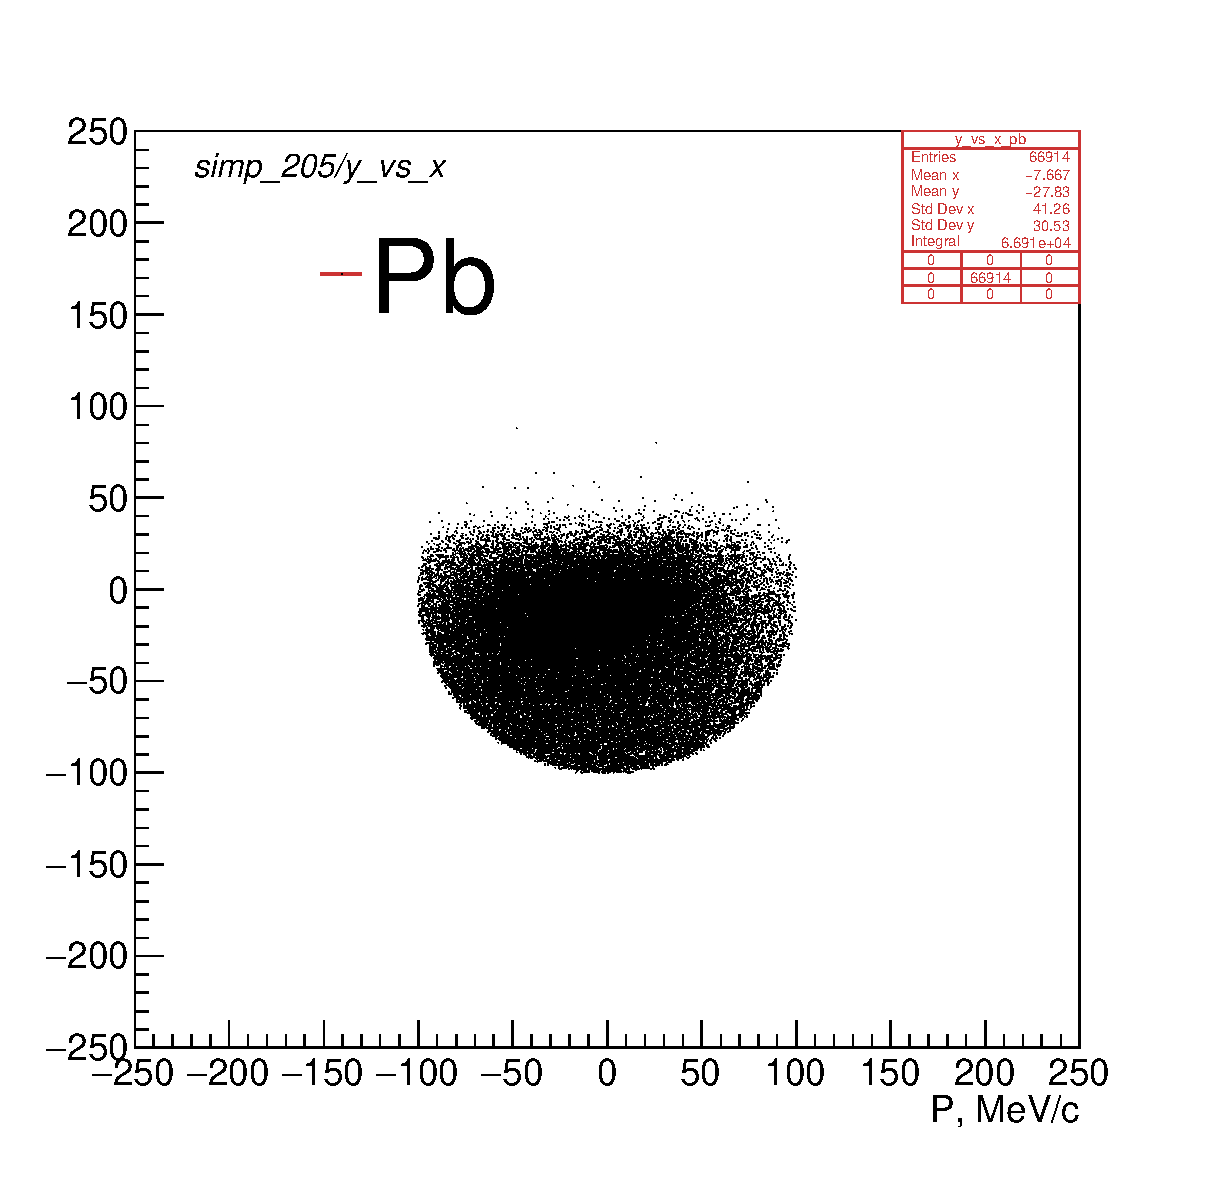
\includegraphics[width=0.5\textwidth]{png/figure_00035}
      %}
    };
    \node[anchor=south west,inner sep=0] at (0,-10.) {
      % \node[shift={(0 cm,0.cm)},inner sep=0,rotate={90}] at (0,0) {}
      % \makebox[\textwidth][c] {
        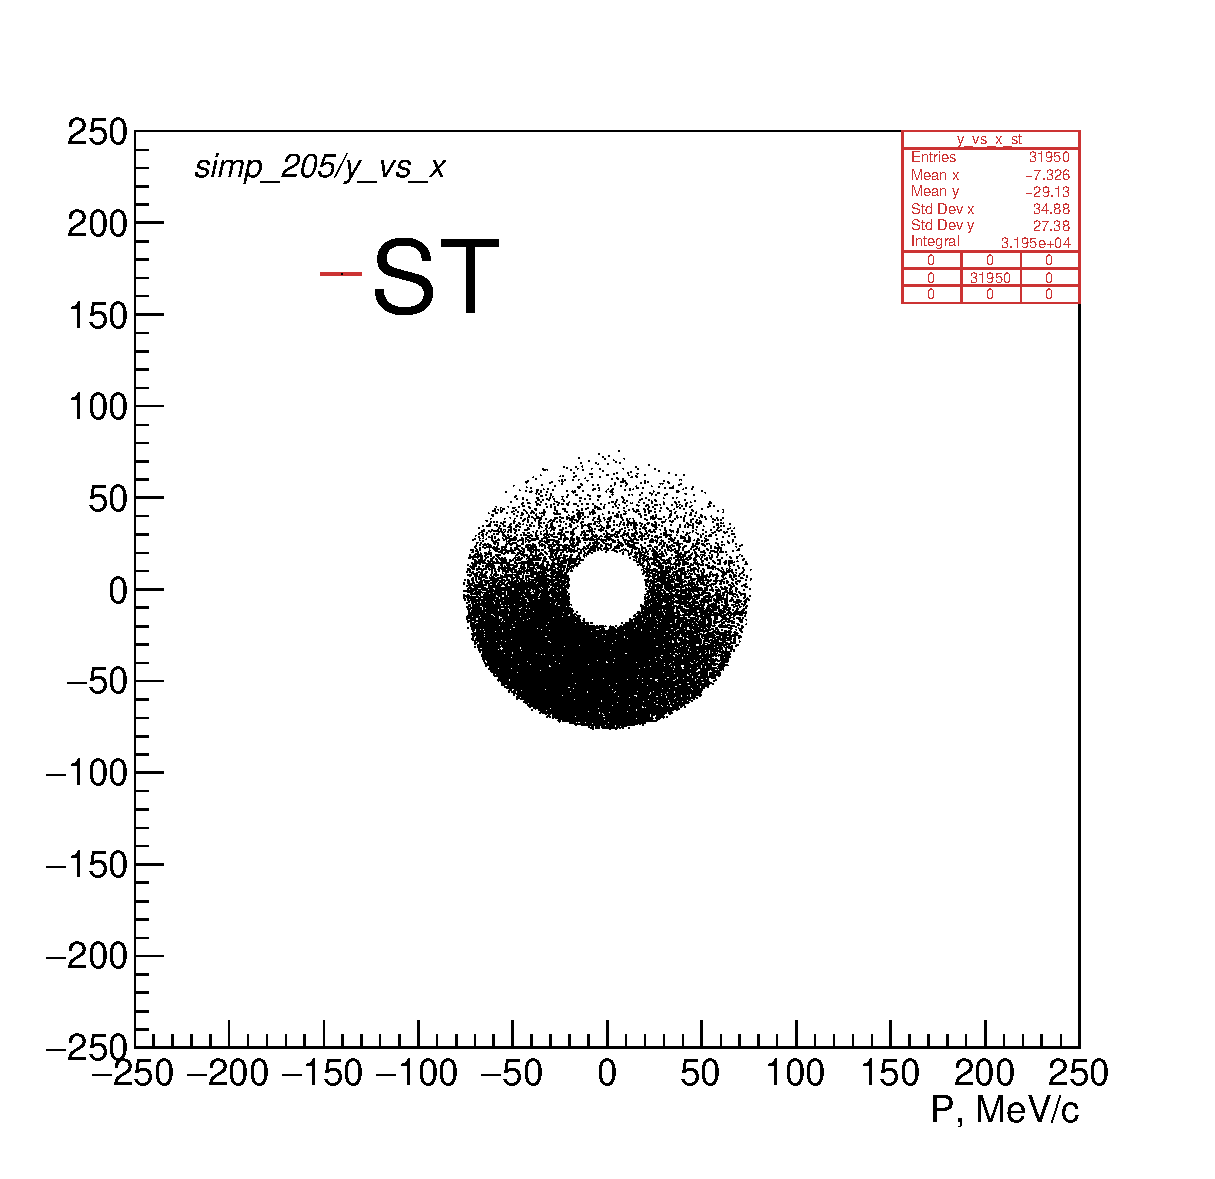
\includegraphics[width=0.5\textwidth]{png/figure_00031}
      % }
    };
    % \node [text width=8cm, scale=1.0] at (14.5,0.5) {$\mu_B$, expected background mean};
    % \node [text width=8cm, scale=1.0, rotate={90}] at (1.5,7.5) { $S_{D}$, ``discovery'' signal strength  };
  \end{tikzpicture}
  \caption{
    \label{figure:y_vs_x_st}
    Y(stop):X(stop) for pions stopped in the CH2, Pb, and ST
  }
\end{figure}


%%% Local Variables:
%%% mode: latex
%%% TeX-master: t
%%% End:
